\documentclass[a4paper]{article}

\usepackage[utf8]{inputenc}
\usepackage[T1]{fontenc}
\usepackage{textcomp}
\usepackage[german]{babel}
\usepackage{amsmath, amssymb, amsthm}
\usepackage{thmtools}
\usepackage{graphicx}


% figure support
\usepackage{import}
\usepackage{xifthen}
\pdfminorversion=7
\usepackage{pdfpages}
\usepackage{transparent}
\usepackage{colonequals}
\newcommand{\incfig}[1]{%
    \def\svgwidth{\columnwidth}
    \import{./figures/}{#1.pdf_tex}
}

\usepackage{setspace}
\setstretch{1.5}

\declaretheorem[style=plain,numberwithin=section, shaded={rulecolor=Black,rulewidth=0.5pt,margin=0.5em,bgcolor={rgb}{1,1,1}}]{satz}
\declaretheorem[style=plain,numberlike=satz]{proposition}
\declaretheorem[style=plain,numberlike=satz]{lemma}
\declaretheorem[style=plain,numberlike=satz]{korollar}

\declaretheorem[style=definition,numberlike=satz, shaded={rulecolor=Black,rulewidth=0.5pt,margin=0.5em,bgcolor={rgb}{1,1,1}}]{definition}
\declaretheorem[style=definition,numberlike=satz]{beispiel}
\declaretheorem[style=definition,numberlike=satz]{bemerkung}
\declaretheorem[style=definition,numbered=no]{erinnerung} \declaretheoremstyle[ spaceabove=-6pt,
spacebelow=6pt,
headfont=\normalfont\bfseries,
bodyfont = \normalfont,
postheadspace=1em,
qed=$\blacksquare$,
headpunct={:}]{myproofstyle} %<---- change this name
\declaretheorem[name={Beweis}, style=myproofstyle, unnumbered]{beweis}

\newcommand{\R}{\mathbb{R}}
\newcommand{\Q}{\mathbb{Q}}
\newcommand{\N}{\mathbb{N}}
\newcommand{\Z}{\mathbb{Z}}
\newcommand{\O}{\varnothing}
\newcommand*{\longeq}{\ratio\Longleftrightarrow}

\renewcommand{\labelenumi}{\roman{enumi})}

\pdfsuppresswarningpagegroup=1

\begin{document}
    \section{Normalteiler}
    \begin{definition}
        Sei $(G, \circ)$ eine Gruppe und $U \subset G$ eine Untergruppe. \\
        H heißt Normalteiler
        \begin{align*}
        &\longeq \forall g \in G \; \forall u \in U: g \circ u \circ g^{-1} \in U
        .\end{align*}    
    \end{definition}
    Der Sauberheit halber müsste das nächste Lemma ausgeführt werden, aber wenn die Zeit zu knapp ist sollte es weggelassen und in die Definition mit aufgenommen werden.
    \begin{lemma}
        Definiere die Verknüpfung von Elementen und Mengen: 
        \[
        x \circ A \circ y = \{x \circ a \circ y  \mid a \in A\}
        .\] 
        Dann ist H Normalteiler in G genau dann, wenn
        \begin{align*}
            &\phantom{\iff} \forall g \in G: g U g^{-1} = U \\
            &\iff \forall g \in G: g U = U g
        .\end{align*}
    \end{lemma}

    \begin{beweis}
        \begin{itemize}
            \item \underline{,,$\implies$''}: \\
                    Es gilt $\forall g \in G \; \forall u \in U: g \circ u \circ g^{-1} \in U$, also $g U g^{-1} \subset U$. \\
                    Ohnehin gilt $U \subset g U g^{-1}$, denn $\forall u \in U: u = e \circ u \circ e ^{-1} \in g U g^{-1}$.
                \item \underline{,,$\impliedby $''}: \\
                    Es gilt $\forall g \in G: g U g ^{-1} \subset U$, also per Definition $\forall g \in G \; \forall u \in U: g \circ u \circ g ^{-1} \in U$.
        \end{itemize}
        Weiterhin gilt
        \[
        g U g^{-1} = U \iff g U g^{-1} g = U g \iff g U = U g
        .\] 
    \end{beweis}

    \begin{beispiel}
        Einige Beispiele für Normalteiler:
        \begin{itemize}
            \item Die triviale Untergruppe $\{e\} $ ist immer Normalteiler, denn es gilt für alle $g \in G: g \circ \{e\} = \{g\} = \{e\} \circ g$.
            \item G ist immer Normalteiler in sich selbst, denn es gilt $\forall g \in G \; \forall g' \in G: g \circ g' \circ g^{-1} \in G$.
           \item Ist G kommutativ, so ist jede Untergruppe $U \subset G$ Normalteiler, denn es gilt $\forall g \in G \; \forall u \in U: g \circ u \circ g ^{-1} = g \circ g ^{-1} \circ u = e \circ u = u \in U$.
        \end{itemize}
    \end{beispiel}
    
    # TODO: Faktorgruppe einbauen?

    \section{Normalisator}
    Sei $\left( G, \circ  \right)$ Gruppe, $U \subset G$ Untergruppe. \\
    Im Allgemeinen ist $U$ kein Normalteiler in $G$. Also suchen wir uns eine größtmögliche Untergruppe von $G$, sodass $U$ in dieser Untergruppe Normalteiler ist. \\
    Formal wollen wir eine Untergruppe $V \subset G$ finden, sodass
    \begin{enumerate}
        \item $U \subset V$ ($U$ ist in $V$ enthalten)
        \item $U$ ist Normalteiler in $V$
        \item Ist $V'$ eine weitere Untergruppe von $G$ die i) und ii) erfüllt, so gilt $V' \subset V$. ($V$ ist größtmöglich)
    \end{enumerate}

    \begin{bemerkung}
        $V$ existiert immer. \\
        Ist $U$ Normalteiler in $G$, so wähle $V = G$. \\
        Ist $U$ kein Normalteiler in G, so erfüllt $V' = U$ die ersten beiden Eigenschaften, also lässt sich auch eine größtmögliche Untergruppe $V$ finden, die die ersten beiden Eigenschaften erfüllt.
    \end{bemerkung}

    \begin{definition}
        \[
            N_G(U) := \{g \in G  \mid g U g^{-1} = U\} 
        \] 
        heißt Normalisator von $U$ in $G$.
    \end{definition}

    \begin{satz}
        $N_G(U)$ ist Untergruppe von G und erfüllt die Eigenschaften i) bis iii).
    \end{satz}

    \vspace{2mm}

    \begin{beweis}
        \begin{itemize} 
            \item \underline{Untergruppe:} \\
        Die Assoziativität wird vererbt.

        Es gilt $e \in N_G(U)$, denn $e \in G$ und $e U e^{-1} = e U e = U$.

        Sei $n \in N_G(U)$. Dann gilt
        \begin{align*}
            &\phantom{\iff}\ n U n^{-1} = U \\
            &\iff n^{-1} n U n^{-1} n = n ^{-1} U n \\
            &\iff U = n^{-1} U n
        ,\end{align*}
        also auch $n^{-1} \in N_G(U)$.

        Seien $n_1, n_2 \in N_G(U)$. Dann gilt:
        \begin{align*}
            (n_1 n_2) U (n_1 n_2)^{-1} &= n_1 n_2 U n_2^{-1} n_1^{-1} \\
                                       &= n_1 (n_2 U n_2^{-1}) n_1^{-1} \\
                                       &= n_1 U n_1^{-1} \\
                                       &= U
        ,\end{align*}
        also auch $n_1 \circ n_2 \in N_G(U)$. \\

        Damit ist $N_G(U)$ Untergruppe von $G$. \\
    \item \underline{i)}: \\
        $U$ ist Normalteiler in sich selbst, also gilt $\forall u \in U: u U u^{-1} = U$. Zudem gilt $U \subset G$. Per Definition von $N_G(U)$ folgt sofort $U \subset N_G(U)$. \\
    \item \underline{ii)}: \\
        Es gilt per Definition $\forall n \in N_G(U): n U n^{-1} = U$, d.h. U ist Normalteiler in $N_G(U)$. \\
    \item \underline{iii)}: \\
        Sei $V' \subset G$ eine weitere Untergruppe mit $U \subset  V'$ und sodass $U$ Normalteiler in $V'$ ist. \\
        Sei $v \in V'$. Da $U$ Normalteiler in $V'$ ist, gilt $v U v^{-1} = U$, also per Definition $v \in N_G(U)$. \\
        $\implies V' \subset N_G(U)$.
    \end{itemize}
    \end{beweis}

    \begin{satz}
        Seien $G, U$ und $N_G(U)$ wie gehabt. \\
        Seien ferner $m \in \N$, $x_1, \ldots, x_m \in N_G(U)$ und $u_0, \ldots, u_m \in U$. Dann gilt für ein geeignetes $u \in U$:
        \[
            u_m \circ x_m \circ u_{m-1} \circ x_{m-1} \circ \ldots \circ u_1 \circ x_1 \circ u_0 = x_m \circ \ldots \circ  x_1 \circ u
        .\] 
        Insbesondere: \\
        $x_m \circ \ldots \circ x_1 \in U \implies u_m \circ x_m \circ u_{m-1} \circ x_{m-1} \circ \ldots \circ u_1 \circ x_1 \circ u_0 \in U$.
    \end{satz}

    \begin{beweis}
        Vollständige Induktion.
        \begin{itemize}
            \item \underline{Induktionsanfang ($m=1$):}
                Zu zeigen: $u_1 \circ x_1 \circ u_0 = x_1 \circ u$ für ein geeignetes $u \in U$. \\
                $U$ ist Normalteiler in $N_G(U)$, also gilt $u_1 \circ x_1 = x_1 \circ \hat{u}$ für ein geeignetes $\hat{u} \in U$. Damit gilt 
                \begin{align*}
                    u_1 \circ x_1 \circ u_0 &= x_1 \circ \hat{u} \circ u_0 \\
                                            &= x_1 \circ u
                \end{align*}
                mit $u := \hat{u} \circ u_0 \in U$.

            \item \underline{Induktionsschritt ($m \implies m+1$):}
                Es gilt:
                \begin{align*}
                    &\phantom{=} u_{m+1} \circ x_{m+1} \circ u_m \circ x_m \circ \ldots \circ u_1 \circ x_1 \circ u_0 \\
                    &= u_{m+1} \circ x_{m+1} \circ (u_m \circ x_m \circ \ldots \circ u_1 \circ x_1 \circ u_0) \\
                    &\overset{I.V.}{=}u_{m+1} \circ x_{m+1} \circ (x_m \circ \ldots \circ x_1 \circ u')  \\
                    &= (u_{m+1} \circ (x_{m+1} \circ \ldots \circ x_1)) \circ u' \\
                    &\overset{NT}{=} ((x_{m+1} \circ \ldots \circ x_1) \circ u'') \circ u' \\
                    &= x_{m+1} \circ \ldots x_1 \circ \underbrace{u'' \circ u'}_{=: u} 
                .\end{align*}
                für geeignete $u', u'' \in U$.
        \end{itemize}
    \end{beweis}

    \section{Symmetrische Gruppe}
    Jegliche Operationen, die im Zaubertrick durchgeführt werden, ändern lediglich die Reihenfolge der Karten im Stapel. Zur Modellierung des Tricks genügt es also, die Karten durchzunummerieren. \\
   
    \begin{definition}
    Wir führen Tricks mit $n$ Karten durch und erzeugen beim Mischen Permutationen von  $\{0, \ldots, n-1\}.$ \\
    Die Gruppe aller dieser Permutationen heißt die \textbf{symmetrische Gruppe} $S_n$. Formal lässt sich mit $\Z_n := \{0, \ldots, n-1\}$ jedes Element von $S_n$ als bijektive Abbildung $\phi : \Z_n &\to \Z_n$ identifizieren.
    \end{definition}

    \begin{erinnerung}
        $\Z_n$ wird mit der Addition und Multiplikation modulo $n$ zu einem Ring, dem \textbf{Restklassenring}.
    \end{erinnerung}

    \begin{definition}
        Sei $r \in Z_n$.
         \begin{align*}
           s_r  : \Z_n &\longrightarrow \Z_n \\
            k  &\longmapsto s_r(k) = k + r \mod n
         \end{align*}
         heißt zyklischer Shift. $s_r$ ist bijektiv, also $s_r \in S_n$.
    \end{definition}

    \begin{bemerkung}
        $s_r$ lässt sich interpretieren als
        \begin{itemize}
            \item Die untersten $r$ Karten nach oben zu legen
            \item Die obersten  $n-r$ Karten abzuheben und unter den Stapel zu legen
        \end{itemize}
        \textit{Im Vortrag am Beispiel klar machen (Menge $\{0, \ldots n-1\}$ von unten nach oben aufschreiben und Shift mit z.B. r = 3 anwenden)}
    \end{bemerkung}

    \begin{satz}
        \[
        S := \{s_r  \mid r \in \Z_n\} 
        \] 
        ist kommutative Untergruppe von $S_n$. \\
        Das bedeutet insbesondere: Die Reihenfolge von mehrmaligem Abheben ist egal (Kommutativität), und mehrmaliges Abheben bringt die Karten nicht mehr durcheinander als einmaliges Abheben (Abgeschlossenheit).
    \end{satz}

    \begin{beweis}
        Es gilt (kurz nachrechnen oder am Abheben klarmachen):  
       \[
           s_{r_1} \circ s_{r_2} = s_{r_2} \circ s_{r_1} = (k \mapsto k + r_1 + r_2 \mod n) = s_{r_1 + r_2}
       ,\] 
       womit die Kommutativität und Abgeschlossenheit gezeigt sind. \\
       Zudem $s_{r}^{-1} = s_{-r} = s_{n-r},$ und $id = s_0 \in S$.
    \end{beweis}

    \section{Normalisator von $S$}
    \begin{bemerkung}
        Definiere
        \[
        \begin{align*}
            \phi_a: \Z_n &\longrightarrow \Z_n \\
            k &\longmapsto \phi_a(k) = ak \mod n
        .\end{align*}
        .\] 
        Wann ist $\phi_a$ bijektiv? \\
        Seien $a$ und $n$ teilerfremd. Dann gilt für $k, k' \in \Z_n:$ 
        \begin{align*}
            \phi_a(k) = \phi_a(k') &\iff ak = ak' \mod n \\
                                   &\iff a(k-k') = 0 \mod n \\
                                   &\iff k-k'  = 0 \mod n \\
                                   &\iff k = k'
        .\end{align*}
        Also ist $\phi_a$ injektiv und damit surjektiv (Abbildung zwischen zwei gleichen endlichen Mengen). \\
        Seien nun  $a$ und $n$ nicht teilerfremd. \\
         $\implies \exists t \in \N: a = t \cdot k, n = t \cdot k'$ für geeignete $k, k' \in \N$. Dann gilt
         \begin{align*}
             \phi_a(k') = a k' = t k k' = n k &= 0 \mod n \\
                                              &= \phi_a(0)
        , \end{align*} 
        also ist $\phi_a$ nicht injektiv. \\
        Damit ist gezeigt: $\phi_a \text{ ist bijektiv} \iff $ $a$ und  $n$ teilerfremd.
    \end{bemerkung}

    \begin{definition}
        Seien $a, b \in \Z.$ Definiere 
        \[
        \begin{align*}
            \phi_{a,b}: \Z_n &\longrightarrow \Z_n \\
            k &\longmapsto \phi_{a,b}(k) = ak + b \mod n
        .\end{align*}
        .\] 
    \end{definition}

    \begin{lemma}\label{phi_bij}
        \[
            a, n \text{ teilerfremd} \implies \phi_{a, b} \in S_n
        .\] 
    \end{lemma}
    \begin{beweis}
       Es gilt  $\phi_{a, b}(k) = ak + b \mod n = s_b(ak) = (s_b \circ \phi_a)(k) $. Es gilt $s_b \in S_n$ und $\phi_a \in S_n$ (haben Bijektivität eben gezeigt), also wegen der Abgeschlossenheit von $S_n$:  $\phi_{a, b} \in S_n$. \\ 
    \end{beweis}

    \begin{lemma} \label{phiab-equiv}
        Sei $\phi \in S_n$ bijektiv. Es gilt:
        \begin{align*}
            \exists a \in \Z_n^{*}, b \in \Z_n : \phi = \phi_{a, b}
            \iff \exists a \in \Z_n: \forall k \in \Z_n: \phi(k+1) = \phi(k)+a \mod n
        .\end{align*}
    \end{lemma}

    \begin{beweis}
        \begin{itemize}
            \item \underline{,,$\implies$":} \\
                Es gilt ($k \in \Z_n$ beliebig)
                \[
                    \phi(k+1) - \phi(k) = a(k+1) + b - (ak + b) = a
                .\] 
            \item \underline{,,$\impliedby$":} \\
            Definiere $\phi(0) = b.$ Zeige per Induktion: $\phi = \phi_{a, b}$.
        \begin{itemize}
            \item \underline{Induktionsanfang ($k = 0$)}: \\
                Es gilt $\phi(0) = b = a \cdot 0 + b = \phi_{a, b}(0)$.
            \item \underline{Induktionsschritt ($k \implies k+1$):}
                Es gilt
                \begin{align*}
                    \phi(k+1) &= \phi(k) +  a \mod n \\
                              &\overset{I.V.}{=} \phi_{a,b}(k) + a \mod n \\
                              &= ak + b + a \mod n \\
                              &= a(k+1) + b \mod n \\
                              &= \phi_{a, b}(k+1)
                .\end{align*}
        \end{itemize}
        Da $\phi$ zudem injektiv ist, müssen $a$ und $n$ teilerfremd sein.
        \end{itemize}
    \end{beweis}
    \begin{satz}
        Es gilt
        \[
            N_{S_n}(S) = \{\phi_{a, b}  \mid a, n \in \N \text{ teilerfremd}\} 
        .\] 
    \end{satz}

    \begin{beweis}
        \begin{itemize}
            \item \underline{,,$\supset$":} \\
                Sei $\phi_{a,b}$ beliebig mit $a, n$ teilerfremd. Nach Lemma \ref{phi_bij} gilt dann $\phi_{a,b} \in S_n$.\\
        Ferner gilt für beliebige $s_r \in S, k \in \Z_n:$
        \begin{align*}
            (\phi_{a, b} \circ s_r)(k) &= \phi_{a, b}(k + r) \\
                                       &= a (k+r) + b \mod n \\
                                       &= (ak + b) + ar \mod n \\
                                       &= (s_{ar} \circ \phi_{a, b})(k)
        .\end{align*}
        Also $\phi_{a, b} \circ s_r \circ \phi_{a, b}^{-1} = s_{ar} \in S$. \\
        $\implies \phi_{a, b} \in N_{S_n}(S)$.

    \item \underline{,,$\subset $":} \\
        Sei $\phi \in N_{S_n}(S)$. Dann gilt insbesondere für alle $k \in \Z_n$ mit geeignetem $s_a \in S$:
        \begin{align*}
            &\phantom{\iff} (\phi \circ s_1 \circ \phi^{-1})(k) = s_a(k) \\
            &\iff (\phi \circ s_1)(k) = (s_a \circ \phi)(k) \\
            &\iff \phi(k+1) = \phi(k) + a \mod n
        .\end{align*}
        Mit Lemma \ref{phiab-equiv} folgt die Behauptung.   
    \end{itemize}
    \end{beweis}


    \section{Zauberhafte Folgerung}
    \begin{bemerkung}
    Welcher Mischvorgang muss auf einen aus n Karten bestehenden Kartenstapel angewendet werden, um eine Permutation der Form $\phi_{a,b}$ zu erhalten? 
     \end{bemerkung}
    \begin{enumerate}
    \item Mischvorgang $R_c$: Sei $c \in \mathbb{N}$. Teile die $n$ Karten von links nach rechts auf $c$ Stapel aus. Danach werden die Karten wieder aufgenommen, und zwar von rechts nach links. Nach ganz oben kommt also der am weitesten links liegende Stapel.
    \item Mischvorgang $L_c$: Von links nach rechts austeilen, und auch von links nach rechts aufnehmen.
    \end{enumerate}
    \textit{(Beispiel vorführen)}
    \begin{definition} 
   
    \begin{enumerate}
    \item Sei $c$ ein Teiler von $c - 1$ und $a := (n - 1)/c$. Dann sind $a$ und $n$ teilerfremd und $R_c$ entspricht $\phi_{a,a}$.
    \item Sei $c$ ein Teiler von $c + 1$ und $a := (n + 1)/n$. Dann sind $a$ und $n$ teilerfremd und $L_c$ entspricht $\phi_{-a,-1}$.
    \end{enumerate}
    \end{definition}
    \vspace{2mm}
    \begin{beweis}
    \begin{itemize}
    \item i) Teilerfremdheit folgt aus $ac = n - 1$: \\
	Angenommen $t$ teilt sowohl $a$ als auch $n$. Wir setzen $tk=a$ und $tk'=n$\\
	\begin{align*}
                    n - ac = 1 & \Leftrightarrow tk' - tkc = 1 \\
                   &\Leftrightarrow t(k' - kc) = 1 \\
                   &\Leftrightarrow $t ist Teiler von 1$
                \end{align*}
    Aus der ursprünglichen Reihenfolge der Karten $(0, …,n-1)$ passiert durch $R_c$ folgendes: 
    \begin{figure}[htbp] 
  \centering
     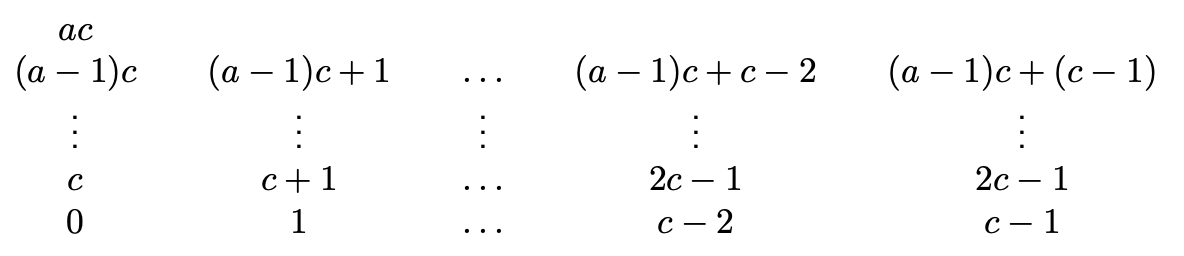
\includegraphics[width=0.7\textwidth]{image1.jpg}
\end{figure} \\
Erster Stapel hat $a+1$ Elemente, alle anderen $a$. \\
$\longrightarrow c$ Stapel von rechts nach links zusammenlegen: \\
Betrachte Karte $k$ aus dem Stapel $s \quad (s \in \lbrace 1, …, c-2\rbrace)$. Dann liegt die Karte $k+1$ im Stapel $s+1$ genau $a$ Stellen weiter als $k$, da in jedem Stapel außer dem ersten genau $a$ Karten sind. In Stapel 1 gilt zusätzlich Karte 0 liegt $a$ Karten weiter als $ac$. \\
Die letzte Karte im Stapel ist $c-1$. Zyklisch weiterzählen. Wir sehen dass Karte $c$ die $a-$te Karte von oben ist. \\
Insgesamt: $R_c(0) = a$ und $R_c(k+1) = R_c(k) + a$. Mit Lemma $4.5$ gilt also $R_c = \phi_{a,a}$.
    \item ii) Teilerfremdheit folgt direkt aus $ac = n+1$. \\
    $ac - n = 1$ $\longrightarrow$ wie vorhin \\
    Aus der ursprünglichen Reihenfolge der Karten $(0, …,n-1)$ passiert durch $L_c$ folgendes: 
    \begin{figure}[htbp] 
  \centering
     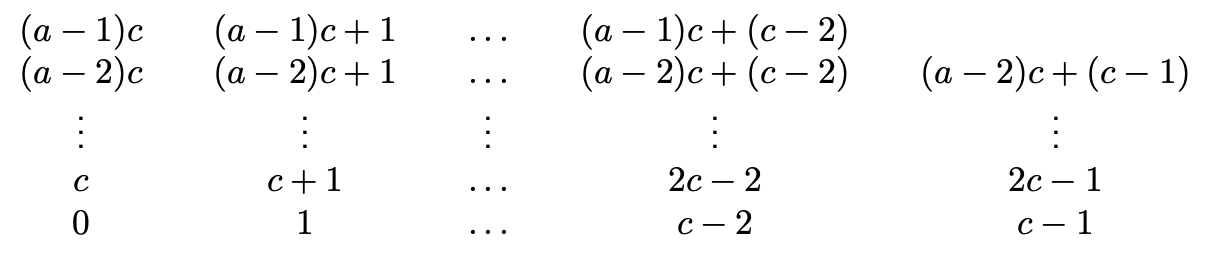
\includegraphics[width=0.7\textwidth]{image2.jpg}
\end{figure} \\
Letzter Stapel hat $a-1$ Elemente, alle anderen $a$. \\
Beweis wie vorhin, aber gehe $a$ Karten zurück um von der Karte $k$ zur Karte $k-1$ zu kommen. Mit $L_c(0) = n-1$ folgt $L_c = \phi_{-a,-1}$. (In $\mathbb{Z}_n$ ist $-1\equiv n-1$). \\
    \textit{Beispiele vorführen}
    \end{itemize}
    \end {beweis}
    \begin{lemma}
   (Schlussfolgerung aus 2.4, 4.5, 5.2) \\
    Für $n \in $ \mathbb{N} sei $A_n := \lbrace x \big\vert \, n-1$ durch $x$ teilbar$\rbrace$ und $B_n := \lbrace x \big\vert \, n+1$ durch $x$ teilbar$\rbrace$. \\
    Wähle $a_1, …. a_r \in A_n$ und $a_1', …, a_l' \in B_n$ aus. Sei $a$ das Produkt aller $a_i$ und $a_j'$. Wähle $c_i$ bzw $c_j'$ sodass $c_ia_i = n-1$, bzw $c_j'a_j' = n+1$. \\
    Führe auf einen Kartenstapel $R_{c_1}, …, R_{c_r}$ und $L_{c_1'}, …, L_{c_l'}$ in beliebiger Reihenfolge durch. Dazwischen darf noch zusätzlich abgehoben werden. Der Kartenstapel befindet sich in der Permutation $\phi_{a,b}$, mit $b$ unbekannt falls abheben beliebig. 
    \end{lemma}
    Wir machen uns klar dass das aus wirklich stimmt: \\
    \begin{align*}
        	R_{c1}R_{c2}(k) &= \phi_{a_1, b_1}  \circ \phi_{a_2, b_2}(k) \\
        	& = \phi_{a_1, b_1}(a_2k + b_2) \\
        	& = a_1(a_2k + b_2) + b_1 \\
        	& = \phi_{a_1a_2, a_1b_2+b_1}(k)
    \end{align*}
    Für uns von Bedeutung: $a=1$ oder $a=-1 \rightarrow$ Die Karten sind in der gleichen, bzw der gespiegelten zyklischen Reihenfolge.
\end{document}
